


% Bounded identity
\begin{frame}{\tciii{} Signed distances}

\begin{columns}
\begin{column}{0.45\linewidth}
\begin{block}{Bounded identity function}
\begin{equation}
\alpha: \begin{cases}
& \text{ if } x \geq 1: \alpha(x) = 1\\ 
& \text{ if } x \leq -1: \alpha(x) = -1\\ 
& \text{ else: }  \alpha(x) = x
\end{cases}
\end{equation}
\end{block}
\end{column}

\begin{column}{0.45\linewidth}
\begin{figure}
\centering
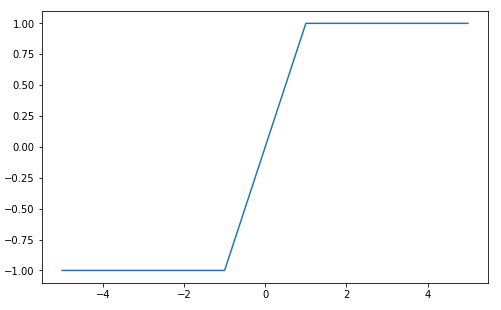
\includegraphics[width=.9\linewidth]{images/GENE/images/bounded.png}
\end{figure}
\end{column}
\end{columns}

\end{frame}


% Final functions
\begin{frame}{\tciii{} Distance functions}

\begin{columns}
\begin{column}{0.60\linewidth}
\begin{block}{pL2-GENE}
\begin{equation}
\alpha \left  ( \prod_{k=1}^D n_1^k - n_2^k \right ) \sqrt{\sum_{j=1}^D \left( n_1^j - n_2^j \right)^2 }
\end{equation}
\end{block}
\end{column}

\begin{column}{0.35\linewidth}
\begin{figure}
\centering
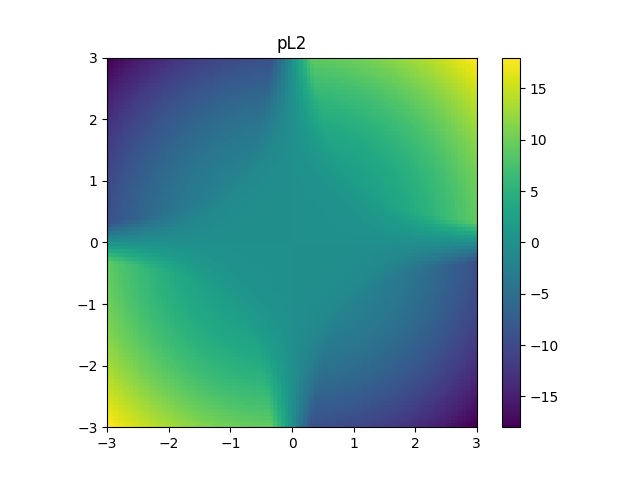
\includegraphics[width=\linewidth]{images/GENE/images/distance_pL2.png}
\end{figure}
\end{column}
\end{columns}

\begin{columns}
\begin{column}{0.60\linewidth}
\begin{block}{tag-GENE}
\begin{equation}
\sum_{j=2}^D \alpha(n_1^j - n_2^1) e^{-|n_1^j - n_2^1|}
\end{equation}
\end{block}
\end{column}

\begin{column}{0.35\linewidth}
\begin{figure}
\centering
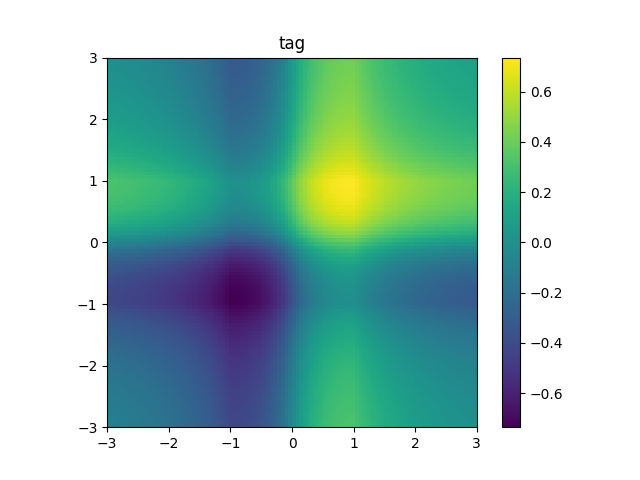
\includegraphics[width=\linewidth]{images/GENE/images/distance_tag.png}
\end{figure}
\end{column}
\end{columns}

\end{frame}


\begin{frame}{\tcv{} The \lucie{} selection procedure}%
    \vspace{1em}
    \onslide<2->{%
        \textbf{Objective:} identify the {\color<2>{cyan}\textbf{best $\mu$}} individuals with as {\color<2>{magenta}\textbf{few evaluations}} as possible.
    }
    \vspace{1em}
    \begin{figure}
        \def\xmax{10}%
        \def\ymax{5}%
        \def\dx{1.3}%
        \def\hicol{magenta}%
        \def\locol{cyan}%
        \def\elcol{green!60!black}%
        \begin{tikzpicture}[%
                ball/.style={circle,inner sep=0,outer sep=0,minimum width=2mm}
            ]%
            % axis
            \onslide<3->{%
                \draw [stealth-stealth,thick] (0,\ymax) node (yaxis) [above] {} |- (\xmax,0) node (xaxis) [right] {};
                \node[rotate=90] at (-0.4,\ymax-0.7) {\textsc{Fitness}};
                \node[] at (\xmax-1.1,-0.4) {\textsc{Individuals}};
            }
            % individuals
            \onslide<4->{%
                \foreach \x in {1,2,3,4,5}{%
                    \node[ball,fill=black,opacity=1.0] at (\x*\dx,0){};
                }
            }
            \onslide<5>{%
                % mean
                \node[] (i1mean) at (1*\dx,2.5) {};
                \node[red] (mean) at (5,4) {\textbf{Empirical mean:} $\hat{f} = \frac{1}{u} \sumc{k=1}{u} y_k$};
                \draw[red,-stealth] (mean.west) to[out=180,in=0] (i1mean.east);
                % ci
                \node[] (i1ci) at (0.1+1*\dx,2.0) {};
                \node[red] (ci) at (5,0.5) {\textbf{Confidence interval:} $\beta(u,t)$};
                \draw[red,-stealth] (ci.west) to[out=180,in=0] (i1ci.east);
                \roundbracket{0.2+1*\dx}{2.0}{0.45}{red}{0.08}{}{90}% x y width color sidesize thickness rotate
            }
            % t=1 fitnesses
            \onslide<5-7>{%
                \only<5>{%
                    \cifit{1*\dx}{2.5}{1}{black} % x y beta color
                    \cifit{2*\dx}{2.4}{1}{black}
                    \cifit{3*\dx}{2.3}{1}{black}
                    \cifit{4*\dx}{2.3}{1}{black}
                    \cifit{5*\dx}{2.1}{1}{black}
                }
                \only<6->{%
                    \cifit{1*\dx}{2.5}{1}{\hicol} % x y beta color
                    \cifit{2*\dx}{2.4}{1}{\hicol}
                    \cifit{3*\dx}{2.3}{1}{\locol}
                    \cifit{4*\dx}{2.3}{1}{\locol}
                    \cifit{5*\dx}{2.1}{1}{\locol}
                }
            }
            % high low sets
            \onslide<6-8>{%
                \node[] at (1.5*\dx,4) {\color{\hicol}\textsc{High}};
                \node[] at (4.0*\dx,4) {\color{\locol}\textsc{Low}};
                \roundbracket{1.5*\dx}{3.8}{0.6*\dx}{\hicol}{0.1}{}{180}
                \roundbracket{4.0*\dx}{3.8}{1.1*\dx}{\locol}{0.1}{}{180}
            }
            % sampling candidates 1
            \onslide<7>{%
                \node[draw, rounded corners=0.1cm] (sc) at (2.5*\dx,-1) {Sampling candidates};
                \draw[-stealth] (sc.north) to[out=90,in=-90] (2*\dx,-0.1);
                \draw[-stealth] (sc.north) to[out=90,in=-90] (3*\dx,-0.1);
                \node[ball,draw,dashed,thick,minimum width=0.5cm] at (2*\dx,1.4) {};
                \node[ball,draw,dashed,thick,minimum width=0.5cm] at (3*\dx,3.3) {};
            }
            % t=2 fitnesses
            \onslide<8>{%
                \cifit{1*\dx}{2.5}{1}{\hicol} % x y beta color
                \cifit{2*\dx}{2.4}{0.7}{\hicol}
                \cifit{3*\dx}{2.3}{0.7}{\locol}
                \cifit{4*\dx}{2.3}{1}{\locol}
                \cifit{5*\dx}{2.1}{1}{\locol}
            }
            % sampling candidates 2
            \onslide<8>{%
                \node[draw, rounded corners=0.1cm] (sc) at (2.5*\dx,-1) {Sampling candidates};
                \draw[-stealth] (sc.north) to[out=90,in=-90] (1*\dx,-0.1);
                \draw[-stealth] (sc.north) to[out=90,in=-90] (4*\dx,-0.1);
                \node[ball,draw,dashed,thick,minimum width=0.5cm] at (1*\dx,1.5) {};
                \node[ball,draw,dashed,thick,minimum width=0.5cm] at (4*\dx,3.3) {};
            }
            % t=3 fitnesses + stop
            \onslide<9->{%
                % stop
                \draw[thick, dashed] (2*\dx,2.3) -- (6*\dx,2.3);
                \draw[thick, dashed] (3*\dx,2.5) -- (6*\dx,2.5);
                \draw[thick] (6*\dx,2.3-0.5) -- (6*\dx,2.5+0.5);
                \draw[thick,-stealth] (6*\dx,2.3-0.5) -- (6*\dx,2.3);
                \draw[thick,-stealth] (6*\dx,2.5+0.5) -- (6*\dx,2.5);
                \node[] at (6.5*\dx,2.4) {$\leq \epsilon$};
                \node[] at (6.5*\dx,3.4) {Stopping Criterion:};
                % sets
                \node[] at (1.5*\dx,4.9) {\color{\hicol}\textsc{High}};
                \node[] at (4.0*\dx,4.9) {\color{\locol}\textsc{Low}};
                \roundbracket{1.5*\dx}{4.7}{0.6*\dx}{\hicol}{0.1}{}{180}
                \roundbracket{4.0*\dx}{4.7}{1.1*\dx}{\locol}{0.1}{}{180}
                % fit
                \cifit{1*\dx}{3.5}{1}{\hicol} % x y beta color
                \cifit{2*\dx}{2.8}{0.5}{\hicol}
                \cifit{3*\dx}{1.8}{0.7}{\locol}
                \cifit{4*\dx}{1.5}{0.5}{\locol}
                \cifit{5*\dx}{1.2}{0.9}{\locol}
                % elite
                \node[ball,fill=\elcol] at (1*\dx,0){};
                \node[ball,fill=\elcol] at (2*\dx,0){};
                \node[] at (1.5*\dx,-0.5) {\color{\elcol}\textsc{Elite}};
                \roundbracket{1.5*\dx}{-0.3}{0.6*\dx}{\elcol}{0.1}{}{0}
            }
        \end{tikzpicture}%
    \end{figure}
\end{frame}


\begin{frame}{\tciv{} DQNES}%
    \begin{figure}
        
    \tikzset{every picture/.style={line width=0.75pt}} %set default line width to 0.75pt        

    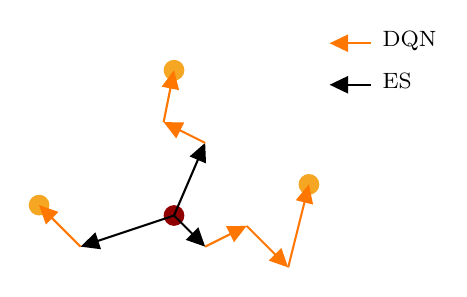
\begin{tikzpicture}[x=0.75pt,y=0.75pt,yscale=-1,xscale=1]
    %uncomment if require: \path (0,300); %set diagram left start at 0, and has height of 300
        % Center
        \onslide<2->{
        %Flowchart: Connector [id:dp7892172092869572] 
        \draw  [draw opacity=0][fill={rgb, 255:red, 145; green, 0; blue, 0 }  ,fill opacity=1 ] (270,155) .. controls (270,152.24) and (272.24,150) .. (275,150) .. controls (277.76,150) and (280,152.24) .. (280,155) .. controls (280,157.76) and (277.76,160) .. (275,160) .. controls (272.24,160) and (270,157.76) .. (270,155) -- cycle ;
        }

        % End points
        \onslide<4->{
        %Flowchart: Connector [id:dp8059049646076628] 
        \draw  [draw opacity=0][fill={rgb, 255:red, 245; green, 166; blue, 35 }  ,fill opacity=1 ] (205,150) .. controls (205,147.24) and (207.24,145) .. (210,145) .. controls (212.76,145) and (215,147.24) .. (215,150) .. controls (215,152.76) and (212.76,155) .. (210,155) .. controls (207.24,155) and (205,152.76) .. (205,150) -- cycle ;
        %Flowchart: Connector [id:dp5011381675096028] 
        \draw  [draw opacity=0][fill={rgb, 255:red, 245; green, 166; blue, 35 }  ,fill opacity=1 ] (270,85) .. controls (270,82.24) and (272.24,80) .. (275,80) .. controls (277.76,80) and (280,82.24) .. (280,85) .. controls (280,87.76) and (277.76,90) .. (275,90) .. controls (272.24,90) and (270,87.76) .. (270,85) -- cycle ;
        %Flowchart: Connector [id:dp3773909027910184] 
        \draw  [draw opacity=0][fill={rgb, 255:red, 245; green, 166; blue, 35 }  ,fill opacity=1 ] (335,140) .. controls (335,137.24) and (337.24,135) .. (340,135) .. controls (342.76,135) and (345,137.24) .. (345,140) .. controls (345,142.76) and (342.76,145) .. (340,145) .. controls (337.24,145) and (335,142.76) .. (335,140) -- cycle ;
        }

        \onslide<3->{
        %Straight Lines [id:da6809885341795275] 
        \draw    (275,155) -- (232.85,169.05) ;
        \draw [shift={(230,170)}, rotate = 341.57] [fill={rgb, 255:red, 0; green, 0; blue, 0 }  ][line width=0.08]  [draw opacity=0] (8.93,-4.29) -- (0,0) -- (8.93,4.29) -- cycle    ;
        %Straight Lines [id:da34929359178134534] 
        \draw    (275,155) -- (288.82,122.76) ;
        \draw [shift={(290,120)}, rotate = 113.2] [fill={rgb, 255:red, 0; green, 0; blue, 0 }  ][line width=0.08]  [draw opacity=0] (8.93,-4.29) -- (0,0) -- (8.93,4.29) -- cycle    ;
        %Straight Lines [id:da4067586836296815] 
        \draw    (275,155) -- (287.88,167.88) ;
        \draw [shift={(290,170)}, rotate = 225] [fill={rgb, 255:red, 0; green, 0; blue, 0 }  ][line width=0.08]  [draw opacity=0] (8.93,-4.29) -- (0,0) -- (8.93,4.29) -- cycle    ;
        %Straight Lines [id:da7752837053635281] 
        \draw    (370,92) -- (353,92) ;
        \draw [shift={(350,92)}, rotate = 360] [fill={rgb, 255:red, 0; green, 0; blue, 0 }  ][line width=0.08]  [draw opacity=0] (8.93,-4.29) -- (0,0) -- (8.93,4.29) -- cycle    ;
        % Text Node
        \draw (374,85) node [anchor=north west][inner sep=0.75pt]  [font=\footnotesize] [align=left] {ES};
        }

        \onslide<4->{
        %Straight Lines [id:da5651183383226251] 
        \draw [color={rgb, 255:red, 255; green, 118; blue, 0 }  ,draw opacity=1 ]   (230,170) -- (212.12,152.12) ;
        \draw [shift={(210,150)}, rotate = 45] [fill={rgb, 255:red, 255; green, 118; blue, 0 }  ,fill opacity=1 ][line width=0.08]  [draw opacity=0] (8.93,-4.29) -- (0,0) -- (8.93,4.29) -- cycle    ;
        %Straight Lines [id:da9174794629852384] 
        \draw [color={rgb, 255:red, 255; green, 118; blue, 0 }  ,draw opacity=1 ]   (290,170) -- (307.32,161.34) ;
        \draw [shift={(310,160)}, rotate = 153.43] [fill={rgb, 255:red, 255; green, 118; blue, 0 }  ,fill opacity=1 ][line width=0.08]  [draw opacity=0] (8.93,-4.29) -- (0,0) -- (8.93,4.29) -- cycle    ;
        %Straight Lines [id:da9236788570029154] 
        \draw [color={rgb, 255:red, 255; green, 118; blue, 0 }  ,draw opacity=1 ]   (310,160) -- (327.88,177.88) ;
        \draw [shift={(330,180)}, rotate = 225] [fill={rgb, 255:red, 255; green, 118; blue, 0 }  ,fill opacity=1 ][line width=0.08]  [draw opacity=0] (8.93,-4.29) -- (0,0) -- (8.93,4.29) -- cycle    ;
        %Straight Lines [id:da5363883614541579] 
        \draw [color={rgb, 255:red, 255; green, 118; blue, 0 }  ,draw opacity=1 ]   (330,180) -- (339.27,142.91) ;
        \draw [shift={(340,140)}, rotate = 104.04] [fill={rgb, 255:red, 255; green, 118; blue, 0 }  ,fill opacity=1 ][line width=0.08]  [draw opacity=0] (8.93,-4.29) -- (0,0) -- (8.93,4.29) -- cycle    ;
        %Straight Lines [id:da8537813572490652] 
        \draw [color={rgb, 255:red, 255; green, 118; blue, 0 }  ,draw opacity=1 ]   (290,120) -- (272.68,111.34) ;
        \draw [shift={(270,110)}, rotate = 26.57] [fill={rgb, 255:red, 255; green, 118; blue, 0 }  ,fill opacity=1 ][line width=0.08]  [draw opacity=0] (8.93,-4.29) -- (0,0) -- (8.93,4.29) -- cycle    ;
        %Straight Lines [id:da4405746369803901] 
        \draw [color={rgb, 255:red, 255; green, 118; blue, 0 }  ,draw opacity=1 ]   (270,110) -- (274.41,87.94) ;
        \draw [shift={(275,85)}, rotate = 101.31] [fill={rgb, 255:red, 255; green, 118; blue, 0 }  ,fill opacity=1 ][line width=0.08]  [draw opacity=0] (8.93,-4.29) -- (0,0) -- (8.93,4.29) -- cycle    ;
        %Straight Lines [id:da8366023954327625] 
        \draw [color={rgb, 255:red, 255; green, 118; blue, 0 }  ,draw opacity=1 ]   (370,72) -- (353,72) ;
        \draw [shift={(350,72)}, rotate = 360] [fill={rgb, 255:red, 255; green, 118; blue, 0 }  ,fill opacity=1 ][line width=0.08]  [draw opacity=0] (8.93,-4.29) -- (0,0) -- (8.93,4.29) -- cycle    ;
        
        % Text Node
        \draw (374,65) node [anchor=north west][inner sep=0.75pt]  [font=\footnotesize] [align=left] {DQN};
        }

\end{tikzpicture}

    \end{figure}
\end{frame}

